\section{Evaluation}

\subsection{Experimental Setup}

\textbf{Implementation of algorithms.}
The algorithms were implemented in C++ code.
The algorithms are built on top of \texttt{einsum\_ir} and use \texttt{torch} for the test setups.
The contractions are hard-coded in the current implementation.

\textbf{Platform.}
The algorithms were tested on a server with an Nvidia Grace CPU Superchip in the Uni Jena and on an AWS g8c.metal-48xl Graviton instance.
All programs were compiled and executed with \texttt{g++} and \texttt{MPICH}.
\texttt{einsum\_ir} was used \texttt{LIBXSMM} and  used \texttt{OpenBLAS} as \texttt{BLAS} routines on Graviton.
On Grace \texttt{einsum\_ir} used Nvidia's \texttt{NVPL BLAS} instead of \texttt{OpenBLAS}.

\textbf{Measurements.}
All measurements show the average result of 10 contractions for each size.
I used Python Matplotlib\cite{matplotlib} to visualize the results.
The JIT Compilation time of \texttt{einsum\_ir} is included in all measurements.


\subsection{Distributed einsum\_ir Performance}

\begin{figure}[ht]
  \centering{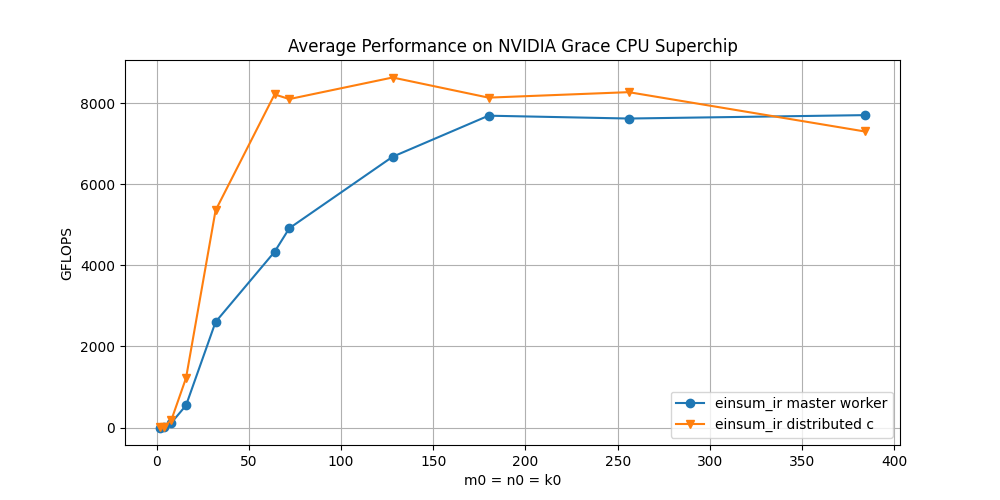
\includegraphics[width=0.5\textwidth]{gflops_grace_master_worker.png}
  }
  \caption{
    Performance of the distributed c-dimension algorithm and the master-worker algorithm on a dual socket NVIDIA Grace CPU Superchip.
    The contraction is $c_0m_0k_0k_1m_1, c_0n_0k_0n_1k_1 \rightarrow c_0m_0n_0n_1m_1$ with $|c_0|=2$, $|m_0|=|n_0|=|k_0|$ and $|m_1|=|n_1|=|k_1|=70$.
    Grace has 72 cores per NUMA domain.
    }
  \label{fig:master_worker_perf}
\end{figure}

First we compare the performance of the master-worker algorithm with the distributed c-dimension algorithm.
We evaluate these algorithms on the einsum expression $c_0m_0k_0k_1m_1, c_0n_0k_0n_1k_1 \rightarrow c_0m_0n_0n_1m_1$.
Figure \ref{fig:master_worker_perf} shows, that the distributed c-dimension algorithm performs significantly better than the master-worker algorithm especially for small tensors.
This is expected since the distributed c-dimension algorithm performs no communication and thus is not slowed down on small tensors by a low compute intensity which suffers more from slower interconnect speeds.
Its advantages diminish the higher the compute intensity is, as seen from $|m_0|=|n_0|=|k_0|= 180$ onwards.
At $|m_0|=|n_0|=|k_0|= 384$ the master-worker algorithm even performs better than the distributed c-dimension algorithm.
I could not test larger sizes as the messages got to big for MPI, which uses a 32-bit signed integer for the element count and due to time constraints I could not rewrite the methods to send multiple smaller messages instead.
The overall result still shows the greater potential in a distributed algorithm, as it can scale easier to more nodes and performs better on most sizes, at least those I could test.
It also places fewer restrictions on the contraction itself, as the distributed c-dimension does not have to be the outermost dimension of all tensors.

\begin{figure}[ht]
  \centering
    \begin{subfigure}[t]{1\textwidth}
      \centering{
        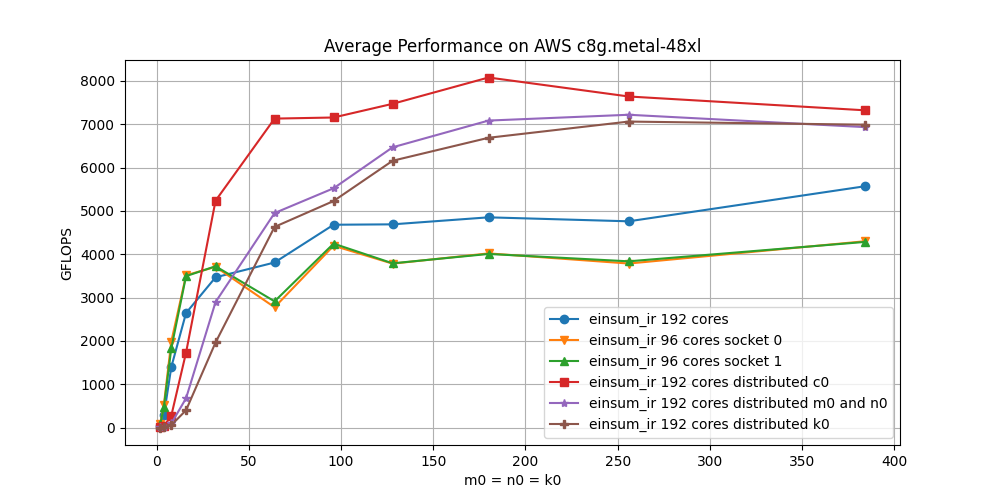
\includegraphics[width=0.49\textwidth]{gflops_g8c.png}
        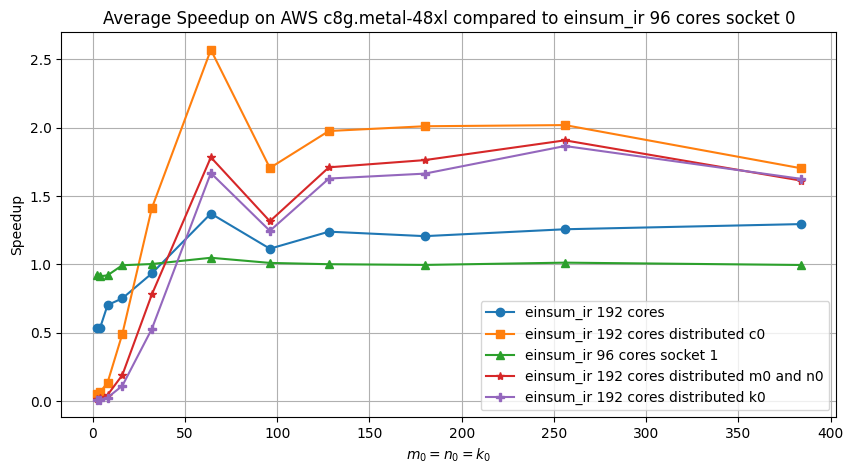
\includegraphics[width=0.49\textwidth]{speedup_g8c.png}
        \subcaption{AWS g8c.metal-48xl}
        \label{fig:einsum_ir_perf_a}
      }
      
    \end{subfigure}
  \centering{
    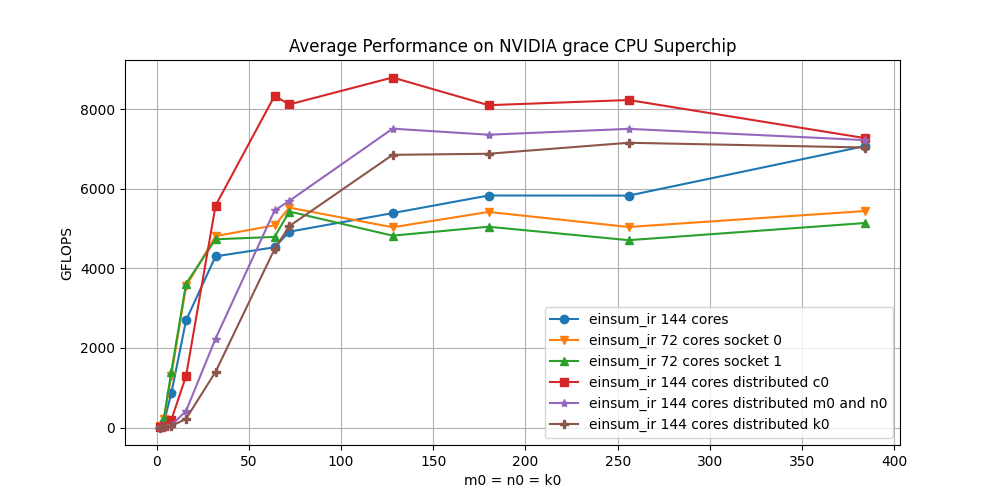
\includegraphics[width=0.49\textwidth]{gflops_grace.png}
    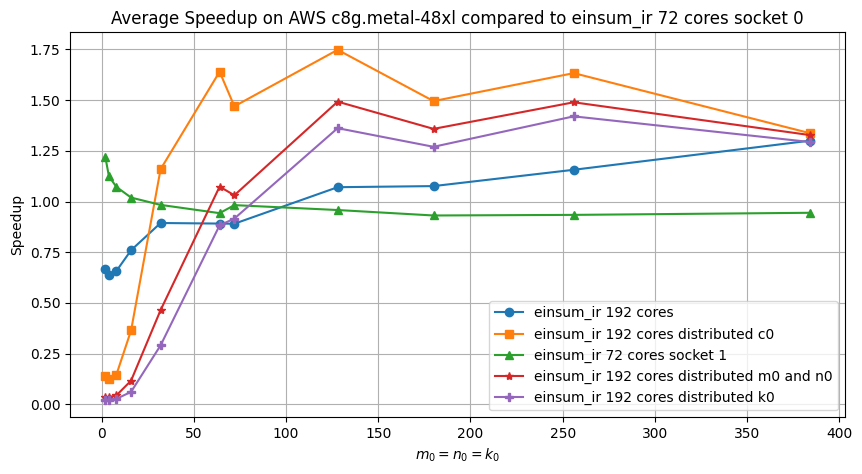
\includegraphics[width=0.49\textwidth]{speedup_grace.png}
    \subcaption{Nvidia Grace CPU Superchip}
    \label{fig:einsum_ir_perf_b}
  }
  \caption{
    Performance and speedup compared to running \texttt{einsum\_ir} on a single socket of various algorithms.
    Tested on a dual socket NVIDIA Grace CPU Superchip (a) and on a dual socket g8c.metal-48xl Graviton AWS instance (b).
    The contraction is $m_0c_0k_0k_1m_1, n_0c_0k_0n_1k_1 \rightarrow m_0n_0c_0n_1m_1$ with $|c_0|=2$, $|m_0|=|n_0|=|k_0|$ and $|m_1|=|n_1|=|k_1|=70\text{ on Grace and } 94\text{ on Graviton}$.
    Grace has 72 cores per NUMA domain; Graviton has 96.
    }
  \label{fig:einsum_ir_perf}
\end{figure}

Next we compare the more general distributed algorithms against each other and the base implementation.
For that we look at the results in Figure \ref{fig:einsum_ir_perf}.
For tensors larger than $|m_0|=|n_0|=|k_0|=128$ we see significant performance improvements of the new distributed memory algorithms over the base shared memory implementation on both Grace and Graviton, except for $|m_0|=|n_0|=|k_0|=384$ on Grace, where shared memory implementation matches the distributed memory's performance.
We also note that for small tensors the distribution harms the performance, which suggests that it could be beneficial contracted small tensors on only one process.
We also observe that in general the distributed c-dimension algorithm performs significantly better than both the distributed m- and n-dimension and the distributed k-dimension algorithms, which are quite close in performance to each other with the distributed k-dimension one being a bit worse.
This is expected since the distributed c-dimension algorithm is the only one of the three algorithms to not have any communication happening and thus never having to run idle waiting for new data and has no synchronization overheads.
The distributed k-dimension algorithm is likely slightly slower than the distributed m- and n-dimension algorithm, since it has double the amount of steps and with that also double the amount of synchronization happening.

It also shows that the second socket on Grace performs about 5\% worse than the first socket.
I am not sure what causes this, but in an earlier measurement all algorithms performed significantly worse on Grace as well, even showing negative speedups in the distributed m- and n-dimension and the distributed k-dimension algorithms.
The difference between those first measurements and the final ones were their runtime.
The first measurements comprised 100 runs for each contraction for all sizes $|m_0|=|n_0|=|k_0|=2,4,...,128$, which made the tests run significantly longer, taking multiple hours per algorithm while the new tests took under an hour for all algorithms combined.
One hypothesis to explain the performance drop would be bad cooling on specifically Grace's second socket, which gets exacerbated the longer the Grace node gets stressed for.
The inclusion of the AWS Graviton instance should show that the algorithms perform well and that the bad initial performance on the Grace node was an outlier.


